The previous sections described how the dispatch parameters passed to a parallel\_for affect how kernels are assigned to GPU processor resources and the software layers and overheads involved in executing a kernel on a GPU. This section describes best practices when a kernel is executing on a GPU.\par

Broadly speaking, kernels are either memory bound, meaning that their performance is limited by data read and write operations into or out of the execution resources on the GPU, or are compute bound, meaning that their performance is limited by the execution resources on the GPU. A good first step when optimizing a kernel for a GPU—and many other processors!—is to determine whether our kernel is memory bound or compute bound, since the techniques to improve a memory-bound kernel frequently will not benefit a compute-bound kernel and vice versa. GPU vendors often provide profiling tools to help make this determination.\par

\begin{tcolorbox}[colback=red!5!white,colframe=red!75!black]
Different optimization techniques are needed depending whether our kernel is memory bound or compute bound!
\end{tcolorbox}

Because GPUs tend to have many processors and wide SIMD widths, kernels tend to be memory bound more often than they are compute bound. If we are unsure where to start, examining how our kernel accesses memory is a good first step.\par

\hspace*{\fill} \par %插入空行
\textbf{Accessing Global Memory}

Efficiently accessing global memory is critical for optimal application performance, because almost all data that a work-item or work-group operates on originates in global memory. If a kernel operates on global memory inefficiently, it will almost always perform poorly. Even though GPUs often include dedicated hardware gather and scatter units for reading and writing arbitrary locations in memory, the performance of accesses to global memory is usually driven by the locality of data accesses. If one work-item in a work-group is accessing an element in memory that is adjacent to an element accessed by another work-item in the work-group, the global memory access performance is likely to be good. If work-items in a work-group instead access memory that is strided or random, the global memory access performance will likely be worse. Some GPU documentation describes operating on nearby memory accesses as coalesced memory accesses.\par

Recall that for our somewhat-parallel matrix multiplication kernel in Figure 15-15, we had a choice whether to process a row or a column of the result matrix in parallel, and we chose to operate on rows of the result matrix in parallel. This turns out to be a poor choice: if one work-item with id equal to m is grouped with a neighboring work-item with id equal to m-1 or m+1, the indices used to access matrixB are the same for each work-item, but the indices used to access matrixA differ by K, meaning the accesses are highly strided. The access pattern for matrixA is shown in Figure 15-17.\par

\hspace*{\fill} \par %插入空行
Figure 15-17. Accesses to matrixA are highly strided and inefficient
\begin{center}
	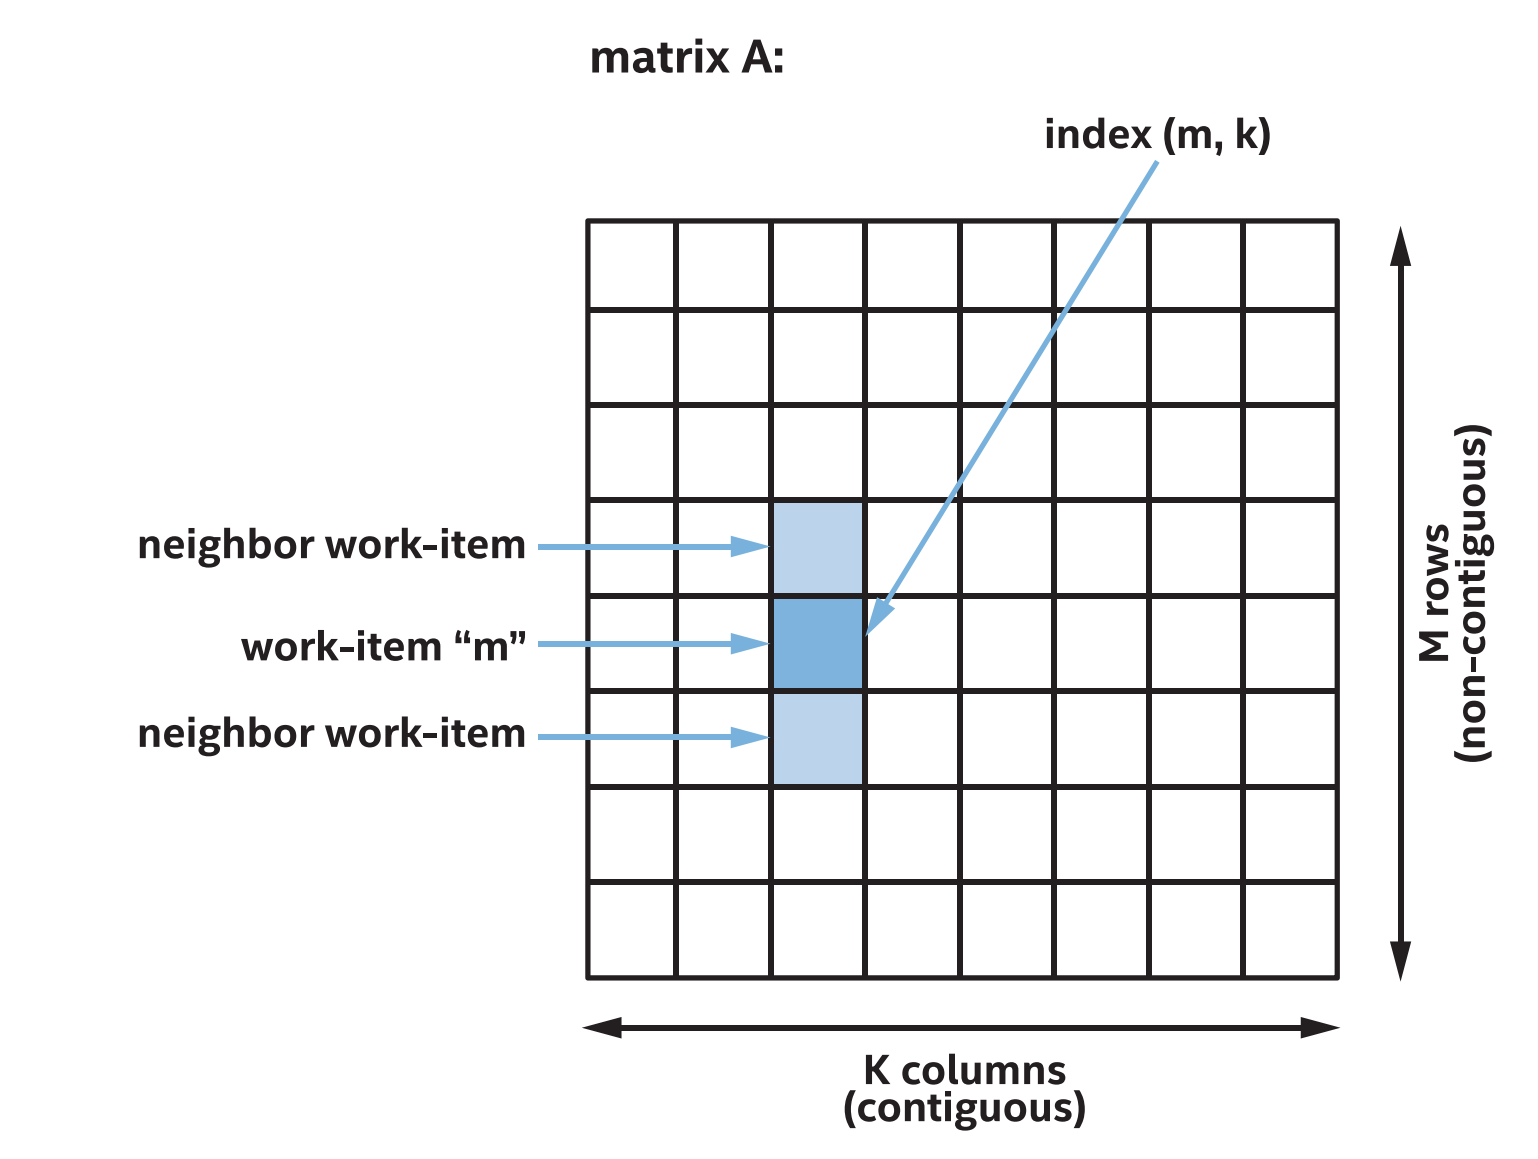
\includegraphics[width=1.0\textwidth]{content/chapter-15/images/13}
\end{center}

If, instead, we choose to process columns of the result matrix in parallel, the access patterns have much better locality. The kernel in Figure 15-18 is structurally very similar to that in Figure 15-5 with the only difference being that each work-item in Figure 15-18 operates on a column of the result matrix, rather than a row of the result matrix.\par

\hspace*{\fill} \par %插入空行
Figure 15-18. Computing columns of the result matrix in parallel, not rows
\begin{lstlisting}[caption={}]
// This kernel processes columns of the result matrix in parallel.
h.parallel_for(N, [=](item<1> idx) {
	int n = idx[0];
	
	for (int m = 0; m < M; m++) {
		T sum = 0;
		for (int k = 0; k < K; k++)
			sum += matrixA[m * K + k] * matrixB[k * N + n];
		matrixC[m * N + n] = sum;
	}
});
\end{lstlisting}

Even though the two kernels are structurally very similar, the kernel that operates on columns of data will significantly outperform the kernel that operates on rows of data on many GPUs, purely due to the more efficient memory accesses: if one work-item with id equal to n is grouped with a neighboring work-item with id equal to n-1 or n+1, the indices used to access matrixA are now the same for each work-item, and the indices used to access matrixB are consecutive. The access pattern for matrixB is shown in Figure 15-19.\par

\hspace*{\fill} \par %插入空行
Figure 15-19. Accesses to matrixB are consecutive and efficient
\begin{center}
	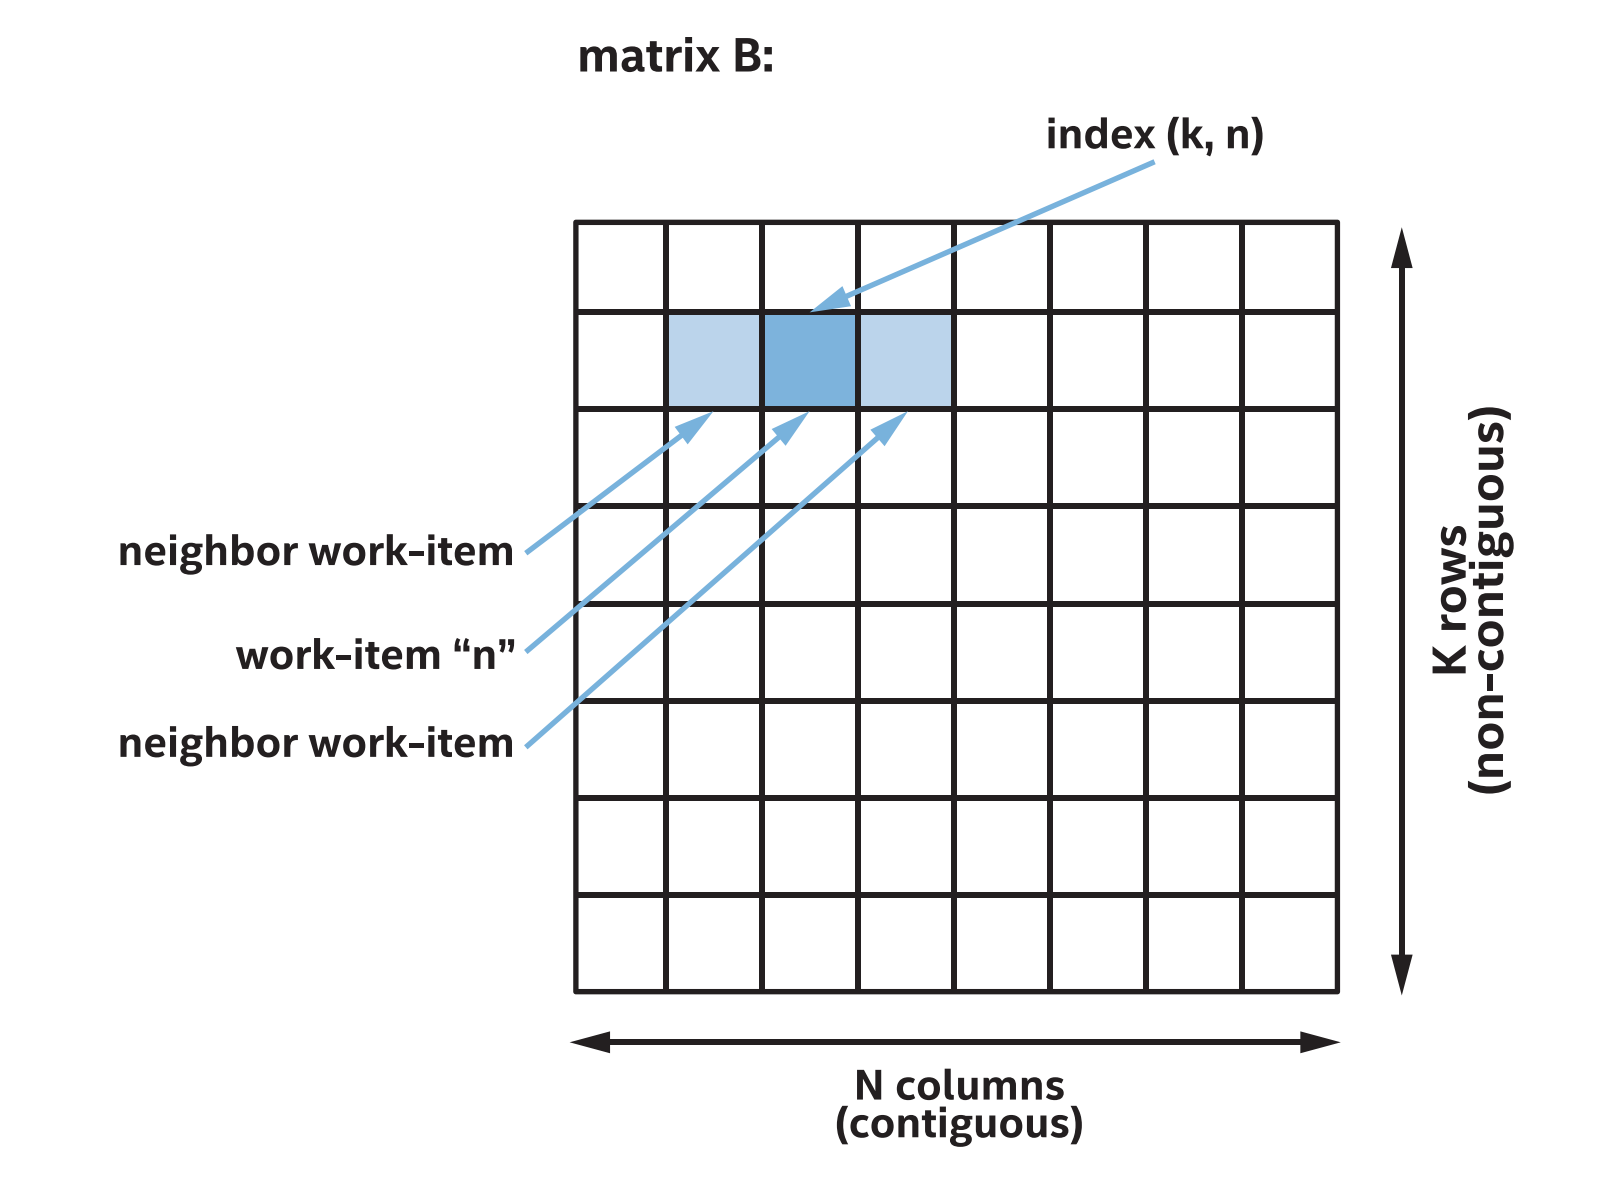
\includegraphics[width=1.0\textwidth]{content/chapter-15/images/14}
\end{center}

Accesses to consecutive data are usually very efficient. A good rule of thumb is that the performance of accesses to global memory for a group of work-items is a function of the number of GPU cache lines accessed. If all accesses are within a single cache line, the access will execute with peak performance. If an access requires two cache lines, say by accessing every other element or by starting from a cache-misaligned address, the access may operate at half performance. When each work-item in the group accesses a unique cache line, say for a very strided or random accesses, the access is likely to operate at lowest performance.\par

\begin{tcolorbox}[colback=blue!5!white,colframe=blue!75!black, title=PROFILING KERNEL VARIANTS]
For matrix multiplication, choosing to parallelize along one dimension clearly results in more efficient memory accesses, but for other kernels, the choice may not be as obvious. For kernels where it is important to achieve the best performance, if it is not obvious which dimension to parallelize, it is sometimes worth developing and profiling different kernel variants that parallelize along each dimension to see what works better for a device and data set.
\end{tcolorbox}

\hspace*{\fill} \par %插入空行
\textbf{Accessing Work-Group Local Memory}

In the previous section, we described how accesses to global memory benefit from locality, to maximize cache performance. As we saw, in some cases we can design our algorithm to efficiently access memory, such as by choosing to parallelize in one dimension instead of another. This technique isn’t possible in all cases, however. This section describes how we can use workgroup local memory to efficiently support more memory access patterns.\par

Recall from Chapter 9 that work-items in a work-group can cooperate to solve a problem by communicating through work-group local memory and synchronizing using work-group barriers. This technique is especially beneficial for GPUs, since typical GPUs have specialized hardware to implement both barriers and work-group local memory. Different GPU vendors and different products may implement work-group local memory differently, but work-group local memory frequently has two benefits compared to global memory: local memory may support higher bandwidth and lower latency than accesses to global memory, even when the global memory access hits a cache, and local memory is often divided into different memory regions, called banks. So long as each work-item in a group accesses a different bank, the local memory access executes with full performance. Banked accesses allow local memory to support far more access patterns with peak performance than global memory.\par

Many GPU vendors will assign consecutive local memory addresses to different banks. This ensures that consecutive memory accesses always operate at full performance, regardless of the starting address. When memory accesses are strided, though, some work-items in a group may access memory addresses assigned to the same bank. When this occurs, it is considered a bank conflict and results in serialized access and lower performance.\par

\begin{tcolorbox}[colback=red!5!white,colframe=red!75!black]
For maximum global memory performance, minimize the number of cache lines accessed.\\
For maximum local memory performance, minimize the number of bank conflicts!
\end{tcolorbox}

A summary of access patterns and expected performance for global memory and local memory is shown in Figure 15-20. Assume that when ptr points to global memory, the pointer is aligned to the size of a GPU cache line. The best performance when accessing global memory can be achieved by accessing memory consecutively starting from a cache-aligned address. Accessing an unaligned address will likely lower global memory performance because the access may require accessing additional cache lines. Because accessing an unaligned local address will not result in additional bank conflicts, the local memory performance is unchanged.\par

The strided case is worth describing in more detail. Accessing every other element in global memory requires accessing more cache lines and will likely result in lower performance. Accessing every other element in local memory may result in bank conflicts and lower performance, but only if the number of banks is divisible by two. If the number of banks is odd, this case will operate at full performance also.\par

When the stride between accesses is very large, each work-item accesses a unique cache line, resulting in the worst performance. For local memory though, the performance depends on the stride and the number of banks. When the stride N is equal to the number of banks, each access results in a bank conflict, and all accesses are serialized, resulting in the worst performance. If the stride M and the number of banks share no common factors, however, the accesses will run at full performance. For this reason, many optimized GPU kernels will pad data structures in local memory to choose a stride that reduces or eliminates bank conflicts.\par

\hspace*{\fill} \par %插入空行
Figure 15-20. Possible performance for different access patterns, for global and local memory
\begin{center}
	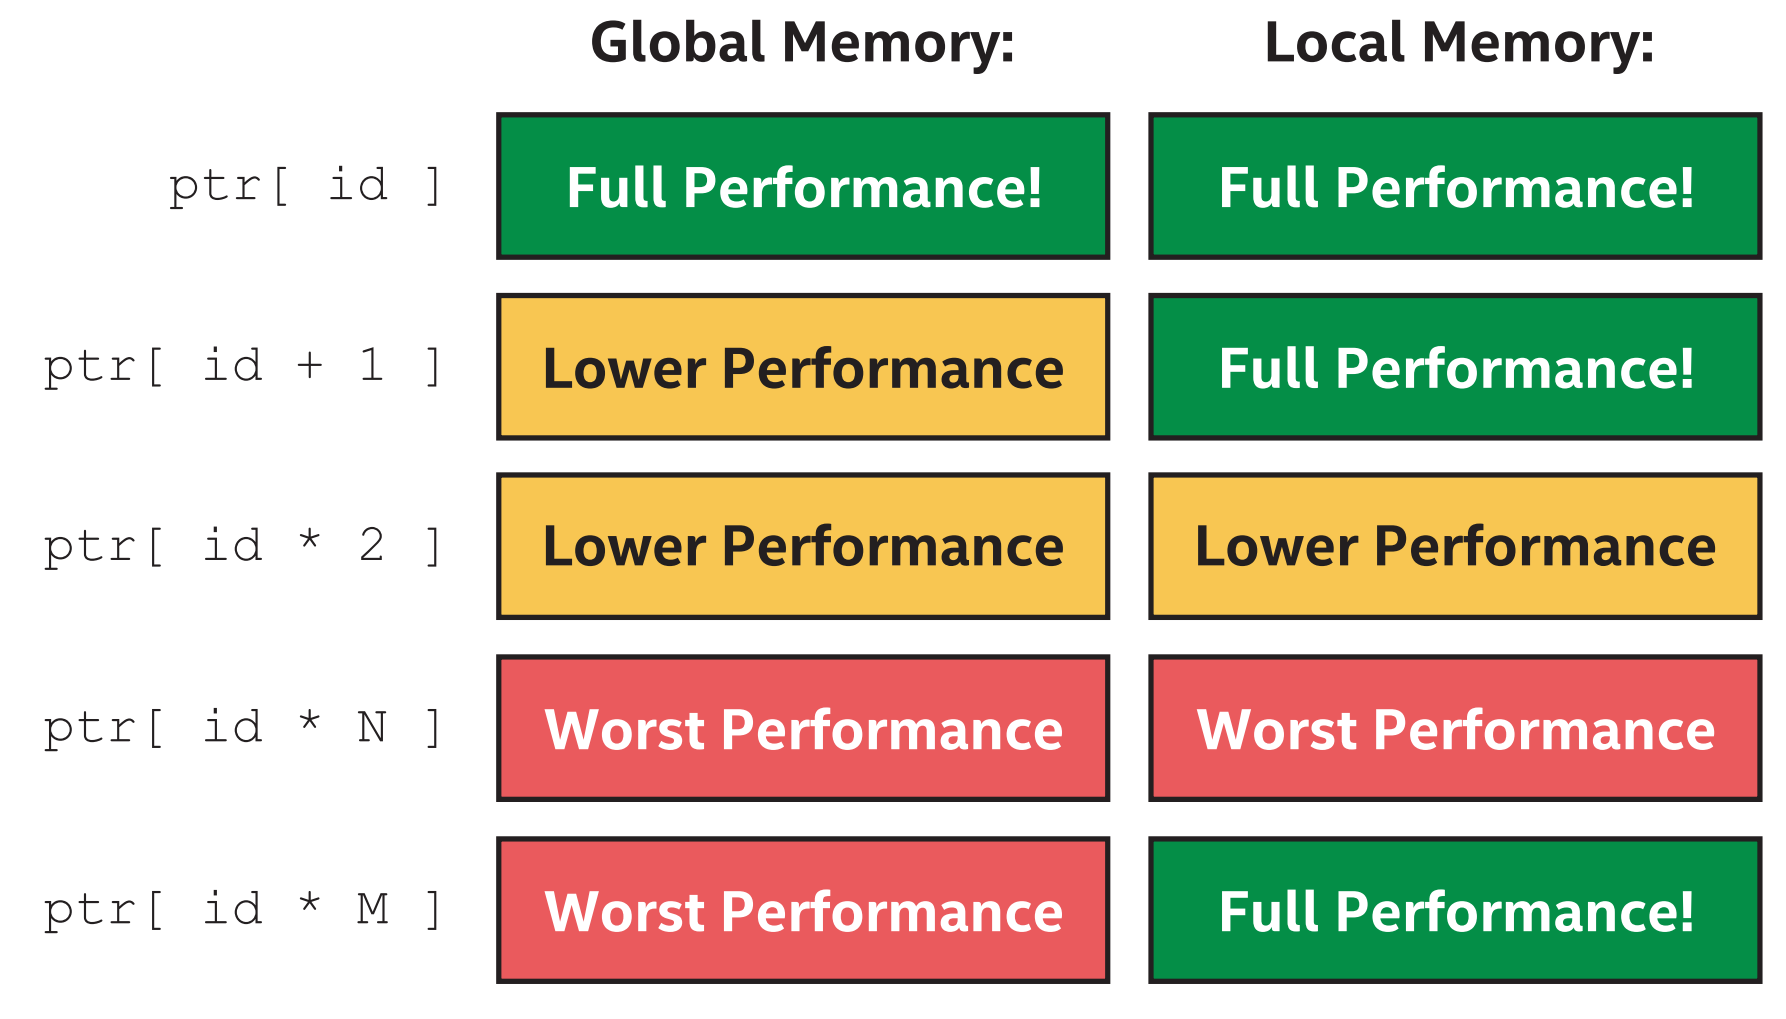
\includegraphics[width=1.0\textwidth]{content/chapter-15/images/15}
\end{center}

\hspace*{\fill} \par %插入空行
\textbf{Avoiding Local Memory Entirely with Sub-Groups}

As discussed in Chapter 9, sub-group collective functions are an alternative way to exchange data between work-items in a group. For many GPUs, a sub-group represents a collection of work-items processed by a single instruction stream. In these cases, the work-items in the sub-group can inexpensively exchange data and synchronize without using workgroup local memory. Many of the best-performing GPU kernels use subgroups, so for expensive kernels, it is well worth examining if our algorithm can be reformulated to use sub-group collective functions.\par

\hspace*{\fill} \par %插入空行
\textbf{Optimizing Computation Using Small Data Types}

This section describes techniques to optimize kernels after eliminating or reducing memory access bottlenecks. One very important perspective to keep in mind is that GPUs have traditionally been designed to draw pictures on a screen. Although pure computational capabilities of GPUs have evolved and improved over time, in some areas their graphics heritage is still apparent.\par

Consider support for kernel data types, for example. Many GPUs are highly optimized for 32-bit floating-point operations, since these operations tend to be common in graphics and games. For algorithms that can cope with lower precision, many GPUs also support a lower-precision 16-bit floating-point type that trades precision for faster processing. Conversely, although many GPUs do support 64-bit double-precision floating-point operations, the extra precision will come at a cost, and 32-bit operations usually perform much better than their 64-bit equivalents.\par

The same is true for integer data types, where 32-bit integer data types typically perform better than 64-bit integer data types and 16-bit integers may perform even better still. If we can structure our computation to use smaller integers, our kernel may perform faster. One area to pay careful attention to are addressing operations, which typically operate on 64-bit size\_t data types, but can sometimes be rearranged to perform most of the calculation using 32-bit data types. In some local memory cases, 16 bits of indexing is sufficient, since most local memory allocations are small.\par

\hspace*{\fill} \par %插入空行
\textbf{Optimizing Math Functions}

Another area where a kernel may trade off accuracy for performance involves SYCL built-in functions. SYCL includes a rich set of math functions with well-defined accuracy across a range of inputs. Most GPUs do not support these functions natively and implement them using a long sequence of other instructions. Although the math function implementations are typically well-optimized for a GPU, if our application can tolerate lower accuracy, we should consider a different implementation with lower accuracy and higher performance instead. Please refer to Chapter 18 for more information about SYCL built-in functions.\par

For commonly used math functions, the SYCL library includes fast or native function variants with reduced or implementation-defined accuracy requirements. For some GPUs, these functions can be an order of magnitude faster than their precise equivalents, so they are well worth considering if they have enough precision for an algorithm. For example, many image postprocessing algorithms have well-defined inputs and can tolerate lower accuracy and hence are good candidates for using fast or native math functions.\par

\begin{tcolorbox}[colback=red!5!white,colframe=red!75!black]
If an algorithm can tolerate lower precision, we can use smaller data types or lower-precision math functions to increase performance!
\end{tcolorbox}

\hspace*{\fill} \par %插入空行
\textbf{Specialized Functions and Extensions}

One final consideration when optimizing a kernel for a GPU are specialized instructions that are common in many GPUs. As one example, nearly all GPUs support a mad or fma multiply-and-add instruction that performs two operations in a single clock. GPU compilers are generally very good at identifying and optimizing individual multiplies and adds to use a single instruction instead, but SYCL also includes mad and fma functions that can be called explicitly. Of course, if we expect our GPU compiler to optimize multiplies and adds for us, we should be sure that we do not prevent optimizations by disabling floating-point contractions!\par

Other specialized GPU instructions may only be available via compiler optimizations or extensions to the SYCL language. For example, some GPUs support a specialized dot-product-and-accumulate instruction that compilers will try to identify and optimize for or that can be called directly. Refer to Chapter 12 for more information on how to query the extensions that are supported by a GPU implementation.\par